\chapter{Electronic and driving circuitry} \label{chapter4}

\section{Power supply} \label{psupply}

In our project, there are three major electronic components which have different power ratings. We have to power an Arduino UNO board, portable mini electric drill and a CNC shield. The Arduino UNO board are often powered via the USB connection or with an external power supply. The power source is selected automatically. External (non-USB) power can come either from an AC-to-DC adapter or battery. The adapter is often connected by plugging a 2.1mm centre-positive plug into the board's power jack. Leads from a battery are often inserted within the GND and Vin pin headers of the source connector. The board can operate an external supply from 6 to 20 volts. If furnished with but  7V, however, the 5V pin could provide but five volts and therefore the board may become unstable. If using quite 12V, the voltage regulator may overheat and damage the board. The recommended range is 7 to 12 volts. The current requirement ranges from 1A - 3A. \par

On the other hand, the electric drill comes in with an attached AC/DC adapter which has an output rating of 9V/1A and is sufficient to rotate the drill bit at nominal speeds. The drill also has manual control for the drill speed (in rpm) which internally adjusts a potentiometer to get the required speed. Similarly, the CNC shield has a rated voltage requirement of 12 - 36 VDC. Now, the problem is to come up with a single (if possible, customised) Power Supply Unit (PSU) which can handle all the devices at once. The 9V rated AC/DC adapter in the electric drill is sufficient to power the Arduino UNO board although it is not even barely sufficient to power the CNC shield (let alone after the current calibration process). At the same time, the current rating of the drill is unknown. Assuming the current rating is in the neighbourhood of 1A (same as the output of the complementary adapter) then splitting its output wires won’t help because the Arduino board won’t receive the expected current for its stable or nominal operation (even if we assume it works in the neighbourhood of the lower bound of the range 1A-3A). These conditions imply that developing a customised PSU for the entire system is very difficult. Even if we use an AC/DC adapter which has a voltage rating of 9V - 12V and a current rating of 1A - 5A with separated output lines it would simply manage to power the Arduino UNO and the electric drill but not the CNC shield. It implies that an adapter having a voltage rating somewhere near 24V will suffice but separate resistors would need to be used (preferably in a voltage divider network) to provide reduced voltage supply to the Arduino UNO board. \par

However, it should be noted that no customised PSU was developed for this project nor were these two electronic components powered by the same unit. The Arduino UNO development board was powered via the USB connection from a laptop while the drill was used along with its complementary AC/DC adapter without any modifications. The CNC shield, on the other hand, was directly powered from a DC regulated power supply.

\begin{figure}[h]
%  \begin{center}
%   \begin{subfigure}{0.5\textwidth}
%   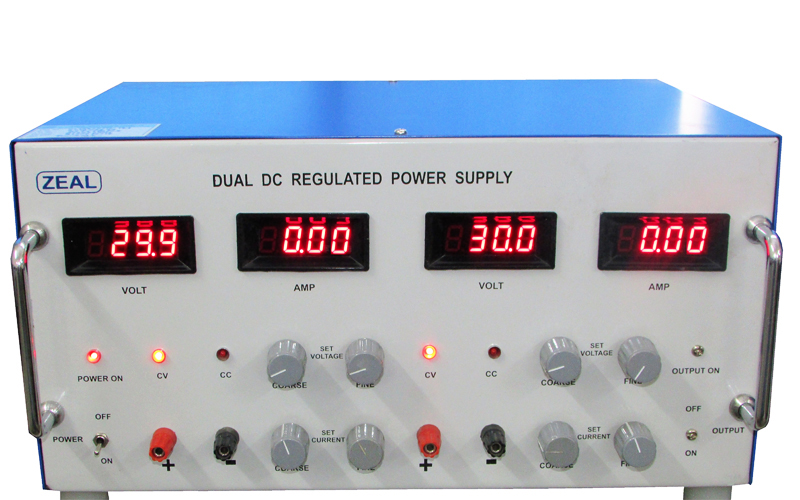
\includegraphics[width=\linewidth, height=6cm]{Chapter_4/dual_dc_regulated_power_supply.jpg}
%   \caption{Dual DC regulated power supply rated at 30V/2A for powering the CNC shield}
%   \label{fig:dc_supply}
%   \end{subfigure} \\
%  \end{center}

 \begin{subfigure}{0.5\textwidth}
  \hspace{5mm}
  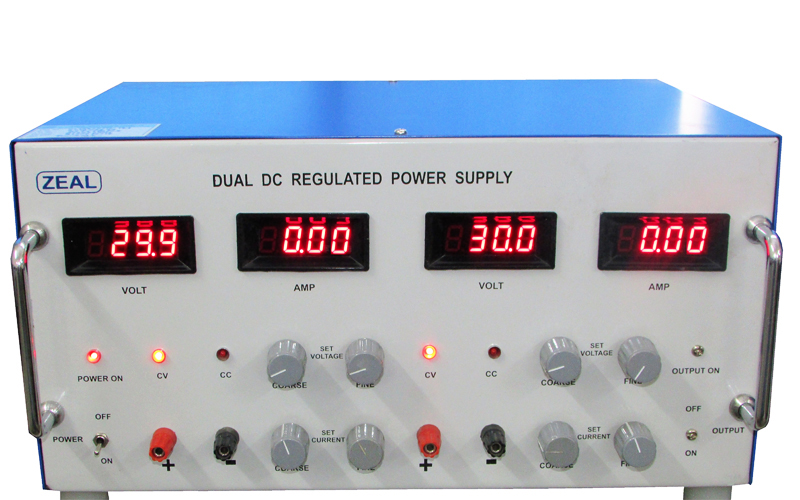
\includegraphics[width=0.9\linewidth, height=6cm]{Chapter_4/dual_dc_regulated_power_supply.jpg}
  \caption{Dual DC regulated power supply rated at 30V/2A for powering the CNC shield}
  \label{fig:dc_supply}
 \end{subfigure}
 \begin{subfigure}{0.5\textwidth}
  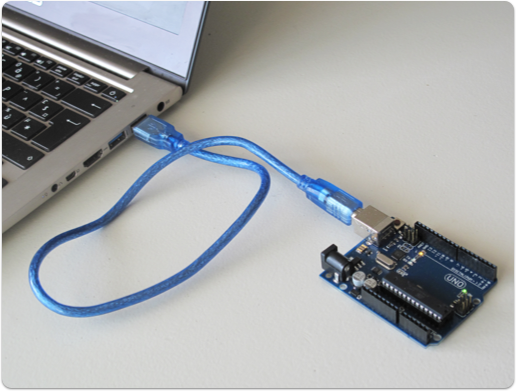
\includegraphics[width=0.9\linewidth, height=6cm]{Chapter_4/arduino_power.png}
  \caption{The Arduino UNO board being powered by USB supply from a laptop}
  \label{fig:arduino_supply}
 \end{subfigure}

 \caption{Various distinct power supplies used in the project (excluding the AC-DC adapter for the electric drill)}
 \label{fig:power_supplies}
\end{figure}

\section{CNC motors}

The most important part of this project is the CNC shield and associated motors. Our project consists of three axes (X-axis, Y-axis and Z-axis) which are controlled by two stepper motors (for X and Y axes) and a single servo motor (for vertical movement of drill bit i.e. Z-axis).

\subsection{Stepper motors} \label{step_motors}

Both X and Y axes are independently controlled by NEMA 17 stepper motors so we require two stepper motors in this project. The stepper motor assigned for the X-axis segment must be able to rotate a coupled rod, resting on which is the entire Y-axis segment (a part of whose weight is resting on this threaded rod and another smooth support rod). So a large capacity stepper motor needs to be considered. If possible, going for a larger capacity stepper motor (say NEMA 23) for the X-axis would ease out the operations in terms of fast and precise movement. \par

The stepper motor for the Y-axis segment is relatively less constrained in terms of weight capacity and any suitable capacity motor which can rotate a threaded rod will do. The NEMA 17 stepper motors used for this project are bipolar i.e. there is only a single winding per phase. The driving circuit must be more complicated to reverse the magnetic pole, this is often done to reverse the current in the winding. However, all that complexity is handled by the dedicated drivers onboard the CNC shield shown in section \ref{cncs}. Following is an illustration of the motor (identical to the one used in the project) followed by a table of its summarised electrical and mechanical specifications.

\begin{figure}[h]
 \centering
 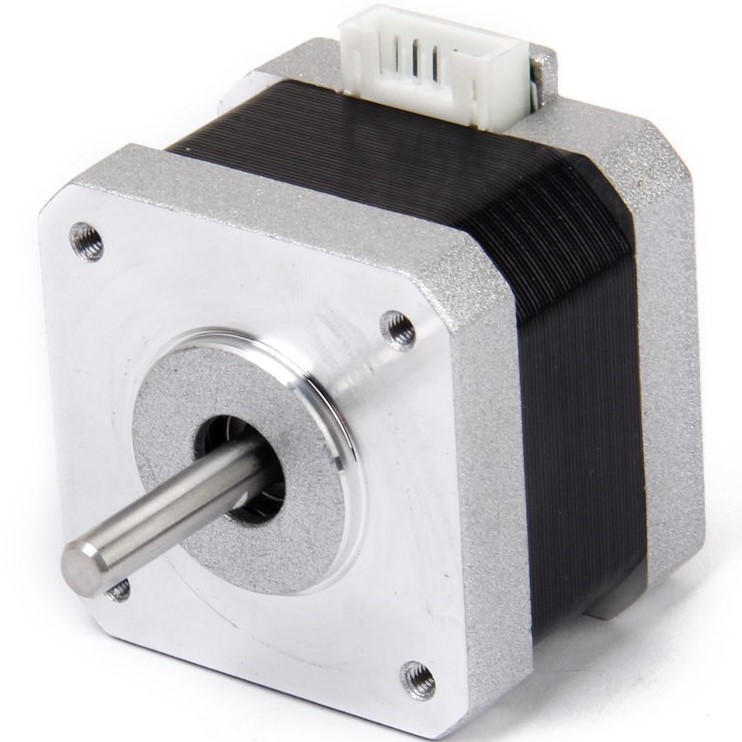
\includegraphics[scale=0.2]{Chapter_4/nema_17.jpg}
 \caption{NEMA 17 stepper motor similar to the one used in the project}
 \label{fig:stepper}
\end{figure}

\begin{table}[h]
 \def\arraystretch{1.5}
 \centering
 \caption{Table of brief specifications of single length NEMA 17 stepper motor}
 \begin{tabular}{|c|c|}
  \hline
  \multicolumn{2}{|c|}{Mechanical specifications} \\
  \hline
  Weight           & 210 g                        \\
  \hline
  Holding torque   & 23 Ncm                       \\
  \hline
  Detent torque    & 1.2 Ncm                      \\
  \hline
  Rotor inertia    & 0.038 kgcm$^{2}$             \\
  \hline
  \multicolumn{2}{|c|}{Electrical specifications} \\
  \hline
  Phase current    & 1.5 A                        \\
  \hline
  Phase resistance & 1.3 $\Omega$                 \\
  \hline
  Phase inductance & 2.1 mH                       \\
  \hline
 \end{tabular}
 \label{tab:step_specs}
\end{table}


\subsection{Servo motor}

The only function of the servo motor of Z-axis is to produce minimal linear actuation of the drill bit (which is attached to the electric drill at its bottom) along the positive and negative Z-axis. Such type of behaviour may be seen when the CNC machine moves from one milling position to another by moving over non-processable space or area on the PCB. For this, we have used a servo motor which can raise the drill bit with gear precision. In terms of G code following is a sample self-explanatory code which may lead to such a movement of the Z-axis.


\begin{flushleft}
 {\fontfamily{qcr}\selectfont G91 (use relative positioning) \\
  G1 Z10 (move z-axis up by 10 mm) \\
  \hspace{18.2mm}(irrespective of initial position)
 }
\end{flushleft}

It should be noted that there are many other equivalent instructions which would produce the same linear actuation. Depending on what the software (described in section \ref{gcodegen}) determines to be feasible in terms of time and space, the appropriate set of G code(s) would be used at the concerning point in the operation of the CNC machine. Following is an illustration of the motor (identical to the one used in the project) followed by a table of its summarised electrical and mechanical specifications.

\begin{figure}[h]
 \centering
 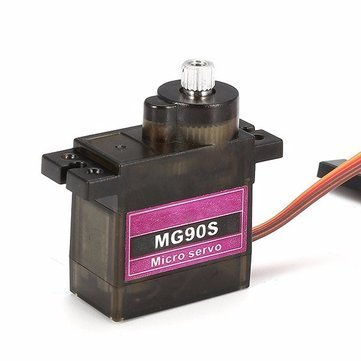
\includegraphics[scale=0.37]{Chapter_4/servo.jpg}
 \caption{Gear precision servo similar to the one used in the project}
 \label{fig:servo}
\end{figure}

\begin{table}[h]
 \def\arraystretch{1.5}
 \centering
 \caption{Table of brief specification of MG90S metal gear servo motor}
 \begin{tabular}{|c|c|}
  \hline
  \multicolumn{2}{|c|}{Mechanical specifications}                           \\
  \hline
  Weight            & 13.4 g                                                \\
  \hline
  Dimensions        & 22.5 $\times$ 12 $\times$ 35.5 mm                     \\
  \hline
  Stall torque      & 1.8 kgf·cm (4.8V ), 2.2 kgf·cm (6 V)                  \\
  \hline
  \multicolumn{2}{|c|}{Electrical specifications}                           \\
  \hline
  Operating speed   & 0.1 s/60$^{\circ}$ (4.8 V), 0.08 s/60$^{\circ}$ (6 V) \\
  \hline
  Operating voltage & 4.8 V - 6.0 V                                         \\
  \hline
  Dead band width   & 5 $\mu$s                                              \\
  \hline
 \end{tabular}
 \label{tab:servo_specs}
\end{table}


\section{Micro controller}

The use of a microcontroller for this specific project is to read the G codes and M-codes and interpret it into corresponding pulses to run the motors. Thus the microcontroller to be used can be of basic specifications. However, it should be noted that the CNC shield should be compatible with the microcontroller development board being used. At the same time, the total cost of the board and the shield shouldn’t exceed the budgetary requirements of the project. \par

Depending on the above conditions we have used an Arduino UNO which is based on ATmega328 microcontroller. A compatible shield for this board is also available in the market. It has 14 digital I/O pins(out of which 6 can be used as PWM outputs and hence major significance in this project), 6 analog inputs and a 16 MHz ceramic resonator (CSTCE16M0V53-R0), a USB connection, an influence(power) jack, an ICSP header, and a reset button. It basically contains everything needed to support a microcontroller, we just simply have to connect it to a computer (or any other programming device having sufficient capabilities and relevant programming software onboard) with a USB cable.

\begin{figure}[h]
 \centering
 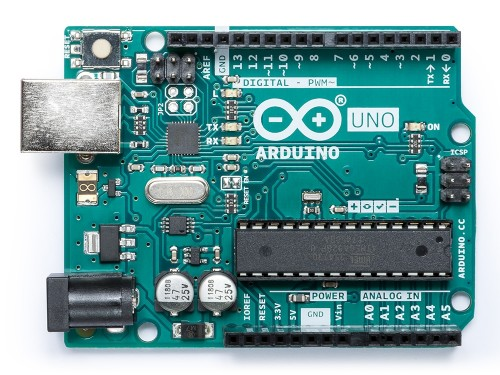
\includegraphics[scale=0.55]{Chapter_4/arduino.jpg}
 \caption{Arduino UNO, the microcontroller used in this project}
 \label{fig:arduino}
\end{figure}

\section{Motor drivers and CNC shield} \label{cncs}

We have to drive three motors (two stepper motors and a single servo motor), for this, we have used a CNC shield. The CNC Shield V3 for Arduino is an Arduino compatible board that turns your Arduino into a CNC controller. Using an open-source firmware it can control up to 4 Stepper motors using DRV8825 or A4988 stepper motor drivers making it easy to get your CNC projects up and running in a few hours. 

\begin{figure}[h]

 \begin{subfigure}{0.5\textwidth}
  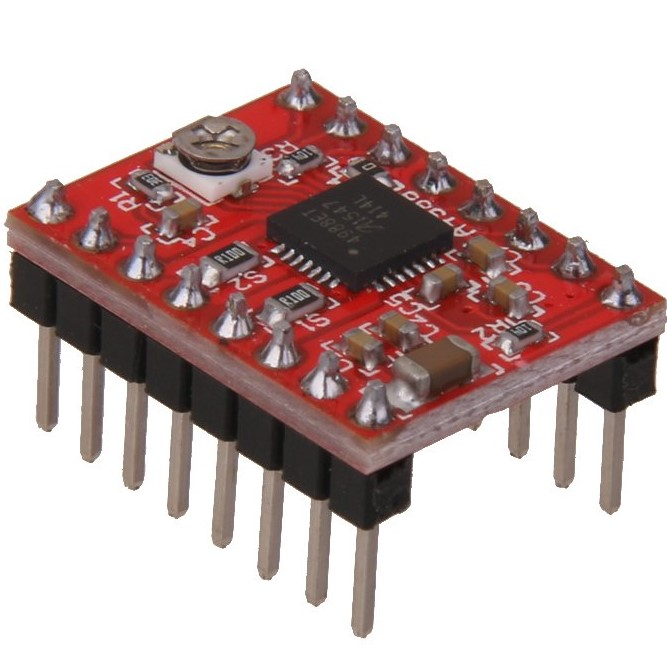
\includegraphics[width=0.8\linewidth, height=6cm]{Chapter_4/motor_driver.jpg}
  \caption{A4988 motor driver}
  \label{fig:motor_driver}
 \end{subfigure}
 \begin{subfigure}{0.5\textwidth}
  \hspace{8mm}
  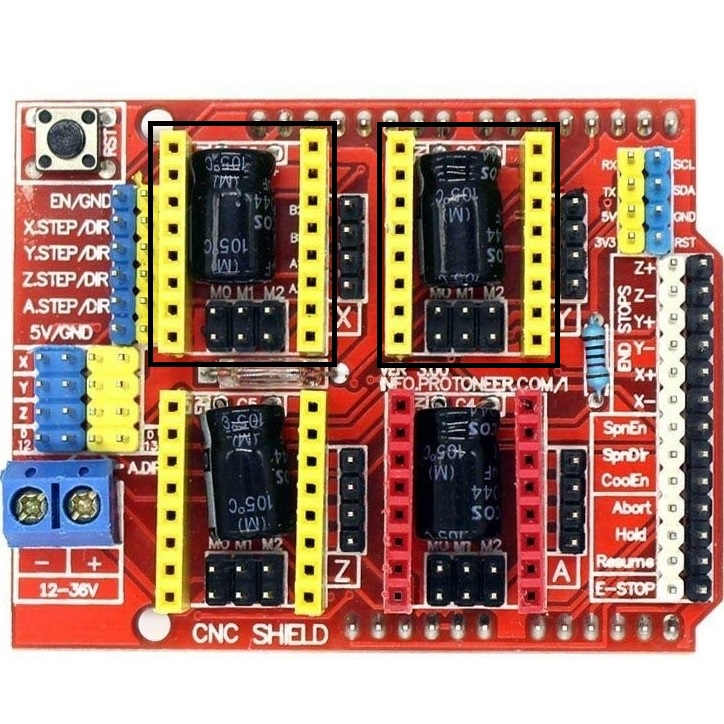
\includegraphics[width=0.8\linewidth, height=6cm]{Chapter_4/cnc_shield}
  \caption{The CNC shield for Arduino used in this project}
  \label{fig:shield}
 \end{subfigure}

 \caption{The two stepper motor drivers are placed in the two slots (indicated in black) on the CNC shield}
 \label{fig:driver_and_shield}
\end{figure}


\section{Heat sinks}

A heat sink is a passive heat exchanger that transfers the heat dissipated from the device to fluid medium, thereby allowing the device to work properly and efficiently without any issues created by the rise in temperature. In our project, it may happen that the driver module heats up due to the load on both the stepper motors. Hence, we have used two heat sinks for the two stepper motors connected via the driver module A4988. The heat sinks (which are standard metallic grills) sit on top of the two motor drivers.

\begin{figure}[h]
 \centering
 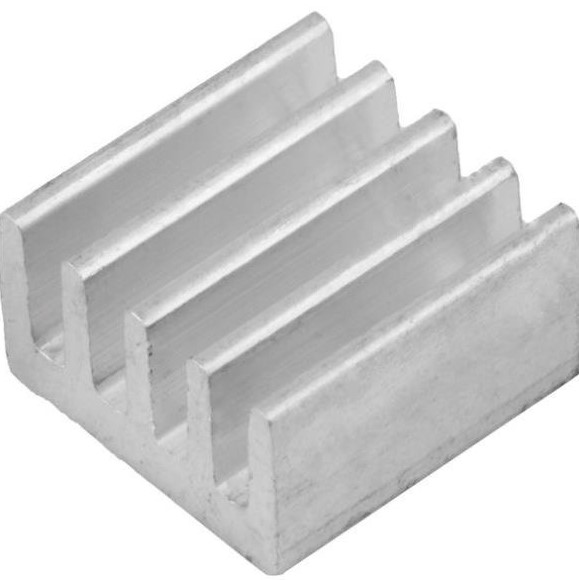
\includegraphics[scale=0.3]{Chapter_4/heat_sink.jpg}
 \caption{Heat sink used for thermal management of the A4988 motor drivers used in this project}
 \label{fig:sink}
\end{figure}


\section{Hardware integration}

In the following subsections, we describe in detail how the hardware interfacing is to be carried out. Apart from that certain calibration steps and standard conventions (in terms of wire colour and selection) have also been discussed at length.

\subsection{Wiring and interfacing} \label{winterface}

The basic advantage of having shields for arbitrary applications related to microcontroller-based development is that it reduces the number and density of the wires required for a particular project or system. As stated before we have selected an Arduino UNO and a compatible CNC shield i.e. the Arduino CNC shield V3. Because of this, there are no wired connections between the microcontroller board and the shield and the shield resides perfectly on top of it by getting directly interfaced to the relevant pins. \par

However, choosing compatible shields has an added disadvantage - the shield completely consumes all of the available pins on the concerned development board. It could be the possibility that \textit{not all pins} available on the development board are of any use in the project or in the functioning of the overall system. However, due to the placement of the shield (on top of the board), there is absolutely no way to access the unused pins heavily affecting effective pin usage and any possible optimisation. This \textbf{\textit{may}} create problems in larger systems and where other supplementary/complementary peripherals may need to be interfaced with the controller. The designer may end up purchasing excess computation units for the project which would again affect budgetary constraints decided for the project.  In this project since there is no need for any additional peripherals other than the one mentioned, choosing a compatible shield for a board turns out to be viable. Following is the pin mapping between the board and the shield for reference. \cite{online_interface_guide} \par

\begin{figure}[h]
 \centering
 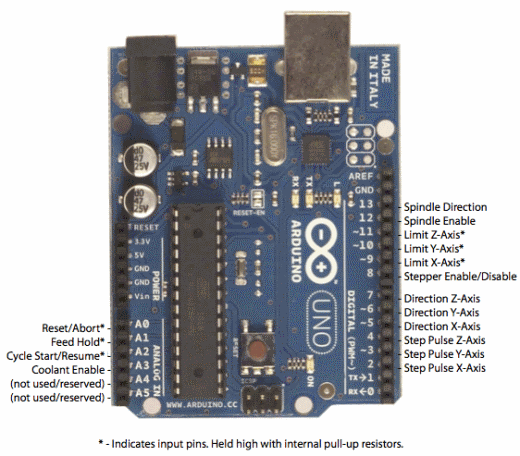
\includegraphics[scale=0.5]{Chapter_4/pin_mapping.png}
 \caption{Pin mapping between the Arduino UNO board and the CNC shield showing the interfacing between the pins from both the modules once they are mounted suitably}
 \label{fig:pin_map}
\end{figure}


Once the CNC shield has been mounted on top of the board we can proceed with attaching the A4988 motor drivers. Now with the reset button (RST) on the top left of the CNC shield (for directional ref.), the pin headers for attaching the motor drivers (in an anti-clockwise sense) are for the X, Y, A and Z axes respectively. Just as seen in the previous case here also we don’t need any separate wires to interface the motor drivers to the shield thereby reducing the number of wires required and the wire interfacing complexity. All three motor drivers are absolutely identical to each other so their choice for the individual axes doesn’t matter. The motor drivers for the X and Y axes are connected to their respective pin headers. These driver chips have extremely small hook-like structures (similar to pins) to attach heat sinks. The heat sinks are to be attached using these structures on to the motor drivers. \par

After these connections have been carried out the motors as well as a suitable DC regulated power supply need to be interfaced with the CNC shield. The stepper motors (corresponding to the X and Y axes) are now to be connected to the motor coils. The connection for the coils on the motor driver is annotated by pins A1, A2, B1 and B2 respectively. It should be noted that the annotation greatly varies across electronic components which are usually interfaced with stepper motors. However, there is no proper annotation on the actual stepper motor so standard wire colour conventions are to be followed. The motor coils (when viewed with all the wire outlets facing the user, starting from left to right) are to be connected to the driver pins according to the following table. \par

\begin{figure}[h]
 \centering
 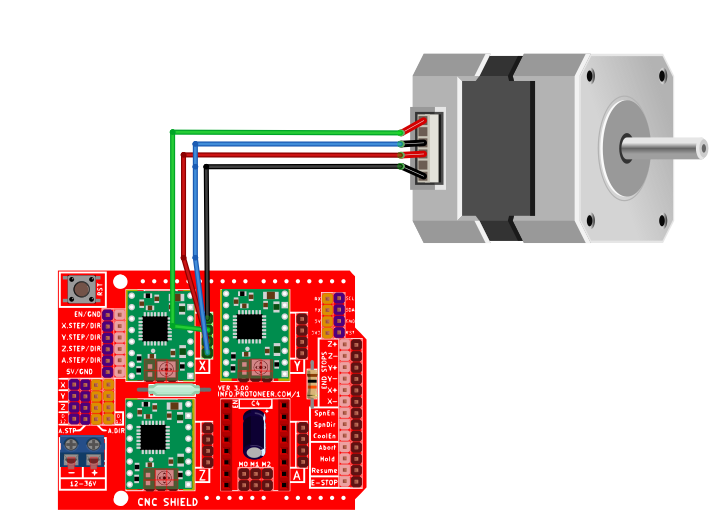
\includegraphics[scale=0.72]{Chapter_4/cnc_stepper.png}
 \caption{Interfacing of a single stepper motor with a corresponding A4988 motor driver mounted on the CNC shield}
 \label{fig:cnc_stepper}
\end{figure}


Since the pin names are quite confusing we have provided a table on the following page for the reference of the reader. It contains the equivalent pin names on the CNC shield, the motor driver and the wires from the stepper motor to be connected to the respective pins. \pagebreak

\begin{table}[h]
 \def\arraystretch{1.5}
 \centering
 \caption{Table of equivalent motor coil connections}
 \begin{tabular}{|c|c|c|c|c|}
  \hline
  Coil pair & Wire colour              & Terminal Annotation & CNC Pin names & Order from Left to Right \\
  \hline
  1         & Black                    & D                   & 2B/B2         & 4                        \\
  \hline
  1         & \textcolor{green}{Green} & B                   & 2A/A2         & 1                        \\
  \hline
  2         & \textcolor{red}{Red}     & A                   & 1A/A1         & 3                        \\
  \hline
  2         & \textcolor{blue}{Blue}   & C                   & 1B/B1         & 2                        \\
  \hline
 \end{tabular}
 \label{tab:mccons}
\end{table}


Interfacing the servo motor (which doesn’t require a driver) to the CNC shield is relatively simple as opposed to interfacing of motors which require the same. The pulse input pin of the servo is interfaced with the \textbf{End stop Z+} pin on the CNC shield (as shown below). The Vcc and the GND pin of the servo motor are interfaced with the 5V and the GND pin on the CNC shield respectively. \par

\begin{figure}[h]
 \centering
 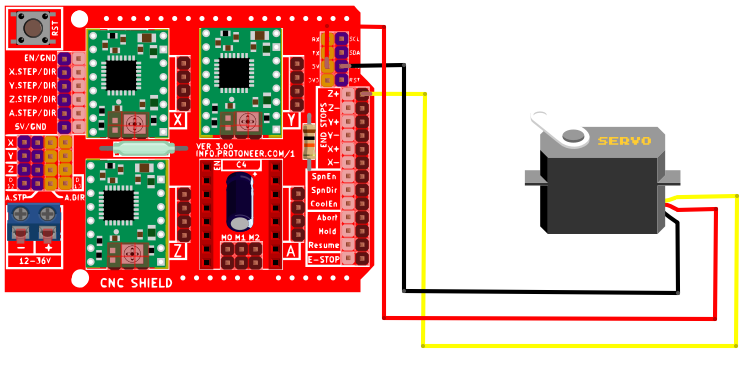
\includegraphics[scale=0.8]{Chapter_4/cnc_servo.png}
 \caption{Interfacing a servo motor with the CNC shield}
 \label{fig:cnc_servo}
\end{figure}

After successfully interfacing the motors to the Arduino board via the CNC shield the board needs to be powered up. To do so it should be noted that the input voltage of Arduino CNC Shield V3.0 is DC 12V-36V, however, the upper bound should be avoided at all costs. The reason being although the input voltage supports power supplies up to 36V the motor drivers interfaced with the same have a supply voltage ($V_{MOT}$) rating of less than 36V. For e.g. the A4988 motor driver used in this project has a supply voltage in the range 8-35V. Using anything outside this range will burn the motor driver. So, the power supply selection should be done carefully after referring to the corresponding motor driver’s datasheet. In our project, a DC regulated power supply rated at a maximum of 30V. In this project voltages in the range of 17V - 20V has been used for powering up the CNC shield. \par

Once the motor assemblies have been wired up to the controller via the CNC shield then the entire setup is now ready to be powered up. However, we still need to calibrate the motor drivers for optimal performance which has been explained in the following section.

Following is the overall circuit of the CNC machine

\begin{figure}[h]
 \centering
 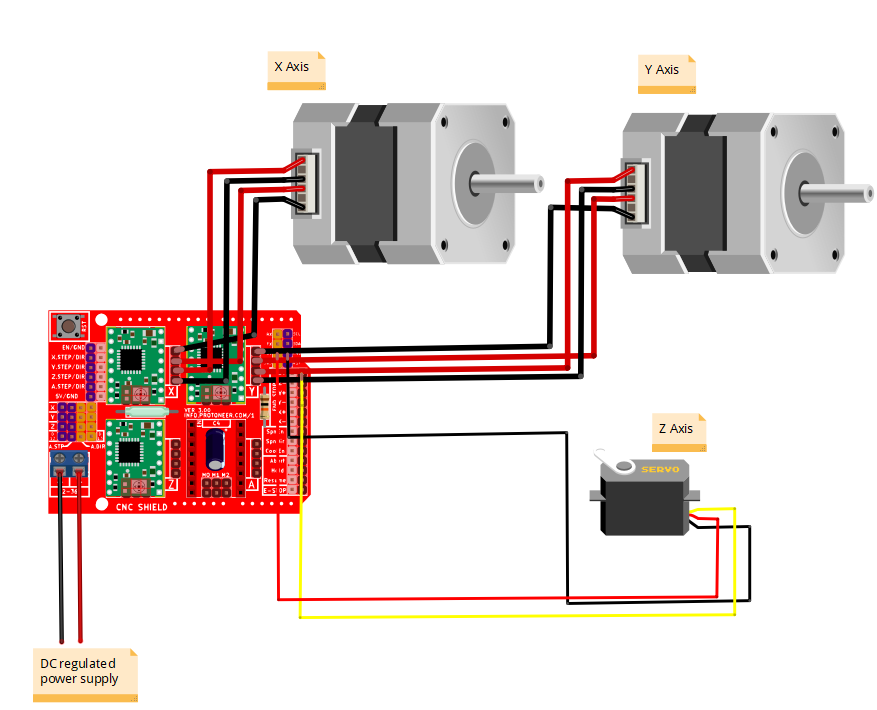
\includegraphics[scale=0.455]{Chapter_4/electronic_circuit.png}
 \caption{Complete electronic circuit for the CNC machine with various motors labelled along with their corresponding axes}
 \label{fig:electronic_circuit}
\end{figure}


\subsection{Motor driver current calibration} \label{motor_calib}

For all CNC based applications, motor driver calibration is an important step before the entire system is powered into normal operation. A slight adjustment to the motor driver is required to ensure that it is not over or under powered. Not over or under powering is important in order to provide the ideal amount of torque for the extruder to run without skipping steps or overheating and damaging the motor. Before proceeding ahead with the calculations it should be noted that there are two types of motors based on their power and capacity used in many CNC based application or CAD/CAM processing in general. They are:

\begin{enumerate}
 \item For the compact but powerful motor, the maximum rated current to be set for stepper driver to output is 1.68A (These motors usually constitute the main electric drill used for engraving or drilling purposes).
 \item For the slimline motor, the maximum rated current to be set for stepper driver to output is 1.4A. (These motors usually constitute the gantry motors i.e. those responsible for the movement of the base and other components of the CNC machine).
\end{enumerate}

There are usually two ways to calibrate the current limiting settings of an A4988 motor driver. Both are described below out of which the latter one is described in more detail and has been used in this project. In both cases, the trimmer potentiometer aboard the motor driver is used in the calibration process.  \cite{online_calib_guide}

\subsubsection*{By measuring the coil current}

One way to line the current limit is to place the driving force into full-step mode and measure the current running through one motor coil while adjusting the current limit potentiometer. This should be through with the motor holding a hard and fast position (i.e. without clocking the STEP input). It should be noted that the current that is being measured is only 70\% of the actual current limit setting since both coils are always on and limited to this value in full-step mode, so if the micro-stepping modes are enabled later, the current through the coils will be able to exceed this measured full-step current by 40\% (1/0.7) on certain steps; This should be taken into account when using this method to set the current limit. Also, it should be noted that this adjustment is to be performed again if the logic voltage is ever changed i.e. $V_{DD}$ since the reference voltage that sets the current limit may be a function of $V_{DD}$. Further, it should also be noted that the coil current can be very different from the power supply current, so the current measured at the power supply shouldn’t be used to set the current limit. Instead, the current meter should be placed is in series with one of the stepper motor coils.

\subsubsection*{By calculating the reference voltage}

\begin{enumerate}
 \item In order to get the accurate result from the subsequent calculation, the value of the resistors used onboard the A4988 motor driver needs to be figured out. Different manufacturers use different resistors which affect the final settable figure. In terms of Pololu A4988's, boards made before Jan 2017 used a Rsense ($R_{CS}$) value of 0.050$\Omega$, boards made after Jan 2017 use a value of 0.068$\Omega$. However, different boards use different values and the same should be verified from the concerned datasheets.In our project we use the variants manufactured before Jan 2017 i.e. those having $R_{CS} = 0.050\Omega$

       \begin{figure}[h]
        \centering
        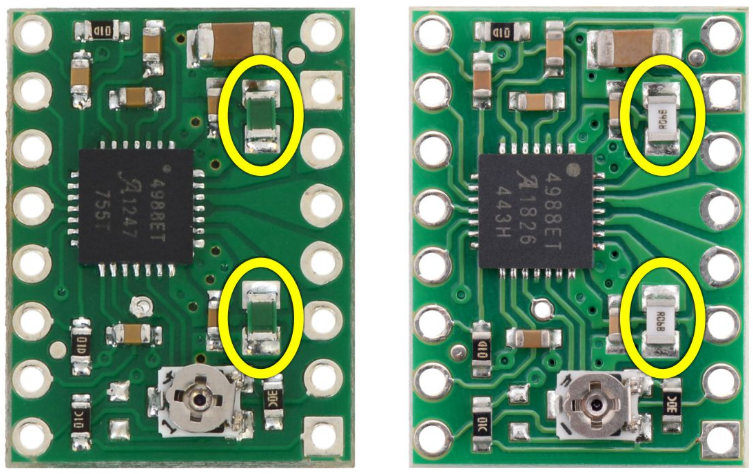
\includegraphics[scale=0.28]{Chapter_4/motor_driver_variants.png}
        \caption{Pololu A4988 motor driver variants (resistors circled in \textcolor{yellow}{yellow}) with  $R_{CS} = 0.050\Omega$ (left) and $R_{CS} = 0.068\Omega$ (right)}
        \label{fig:driver_variants}
       \end{figure}

 \item  The current limit $\boldsymbol{I_{MAX}}$ is related to the reference voltage $\boldsymbol{V_{REF}}$ as follows
       \begin{align}
        \boldsymbol{I_{MAX} = \frac{V_{REF}}{8R_{CS}}} \nonumber
       \end{align}

       Rearranged to solve for $\boldsymbol{V_{REF}}$ we get
       $ \boldsymbol{V_{REF} = 8 \cdot I_{MAX} \cdot R_{CS}}$  where $\boldsymbol{R_{CS}}$ is the sense resistor described above. In this project the decided value of $\boldsymbol{I_{MAX}= 1.7A}$  and value of sense resistor i.e. $\boldsymbol{R_{CS} = 0.050\Omega}$. \\
       Substituting in the above formula we get  $\boldsymbol{V_{REF} = 1.7\times8\times0.050 = 0.68V}$.

 \item  Now a multimeter is to be used for measuring the current value of reference voltage. The 2V DC option is to be set on the multimeter. The CNC shield should not be merely powered by the USB cable rather it should be fully powered to get a correct reading.

       \begin{figure}[h]
        \centering
        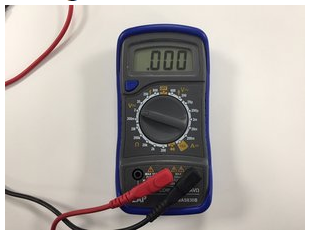
\includegraphics{Chapter_4/correct_options.png}
        \caption{A multimeter with the required options set for calibration}
        \label{fig:correct_options}
       \end{figure}


 \item Now the red and black probes of the multimeter are connected to the potentiometer and the ground pin of the motor driver respectively as shown below.

       \begin{figure}[h]
        \hspace{20mm}
        \begin{subfigure}{0.5\textwidth}
         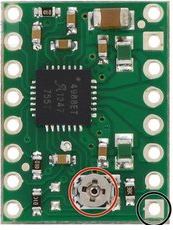
\includegraphics[scale=0.9]{Chapter_4/pins_to_be_probed.png}
         \label{fig:to_be_probed}
        \end{subfigure}
        \hspace{-20mm}
        \begin{subfigure}{0.5\textwidth}
         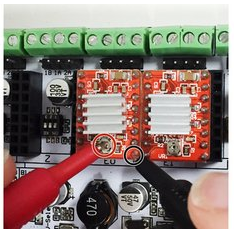
\includegraphics[scale=0.9]{Chapter_4/multimeter_probes.png}
         \label{fig:multimeter_probes}
        \end{subfigure}

        \caption{The points on the driver to be probed encircled in \textcolor{red}{red} and black (left) and multimeter probes of the same colour (right)}
        \label{fig:probes}
       \end{figure}

       % adjust terms like next page, following etc. if any changes occur %

       A ceramic screwdriver should be used in order to rotate the potentiometer to prevent shorting out any of the components whilst performing the adjustment as shown on the following page.

       \begin{figure}[h]
        \centering
        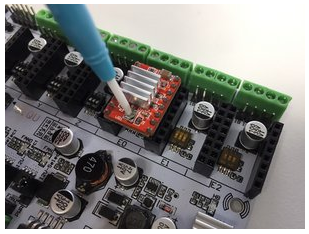
\includegraphics{Chapter_4/ceramic_scredriver.png}
        \caption{A ceramic screwdriver}
        \label{fig:ceramic_scredriver}
       \end{figure}

 \item   The first reading that would be obtained is the current value of the reference voltage (this would be higher or lower than the calculated value in the previous step indicating that the motor may either overheat or won’t be sufficiently powered for nominal performance). On rotating the potentiometer anticlockwise or clockwise the value of reference voltage can be decreased or increased respectively so as to reach the calculated value from the previous step. Depending on the manufacturer of the board the direction of rotation may be different so the same should be checked before turning it too far.

 \item  Correctly setting the potentiometer to the required value (from the multimeter reading) concludes the current calibration process of the motor driver.
\end{enumerate}


\subsection{Wire selection on the basis of component interfacing}

The contents of this section are optional, however, these are some recommended conventions and rules which are ought to be followed so as to develop a properly working self-explanatory system. Before proceeding further it should be noted that the CNC module is directly mounted on the Arduino while the motor drivers are directly mounted on the CNC shield. The heat sinks are fixed onto the motor drivers. Any form of wired connection is \textbf{not needed} for these purposes which further emphasises the advantages of using dedicated microcontroller shields for various applications wherein required.

\subsubsection*{Wires for generic interfacing}
As far as generic interfacing is concerned \textcolor{red}{red} coloured wires are suitable for DC power supply while nornmal black wires are suitable for representing GND or negative terminals. All connections between a single peripheral to the controller should be coloured similarly. For e.g. \textcolor{blue}{blue}. The colour should be changed as soon as we shift to a new peripheral.

\subsubsection*{Wires related to interfacing between motor and CNC shield}

Motor coil wires are connected to dedicated driver pins on the CNC module. However, as stated in section \ref{winterface} there is no form of annotation on the motors indicating which coil is to be connected to what. Additionally, the wires are not labelled in any form indicating their actual electrical significance with the coils (inductor coils) present inside and their order of magnetisation. So the primary, as well as the proper way of identifying the wires, is their colour. In this project, we are using a pair of bipolar stepper motors which have a total of four leads/wires which are actually connected to the internal winding and can be accessed. Since there is only a single winding per phase, reversing the magnetic pole is relatively complicated as opposed to a unipolar stepper motor. However, that complexity is taken care of by using dedicated motor driver chips. \par

The four leads of the stepper motor \cite{online_diff_guide} are customary to be coloured distinctively. In our project, the stepper motor wires are coloured as Red, Blue, Green and Black. The former two belong to the first coil pair and the latter two belong to the second coil pair. An illustrative figure is shown below with all the motor coils alongside the image of all the wires coming out from a stepper motor.

\begin{figure}[h]
 \begin{subfigure}{0.5\textwidth}
  \hspace{9mm}
  \begin{circuitikz}
   \draw (0,0) to[L,l=$C_{1}$,o-o,color=blue] (0,2) to[L,l=$A_{1}$,o-o,color=red] (0,4);
   \draw (0.5,0) to[L,a=$D_{2}$,o-o] (2.5,0) to[L,a=$B_{2}$,o-o,color=green] (4.5,0);
   \draw (2.5,2) node[/tikz/circuitikz/bipoles/length=3.5cm,elmech](motor){M};
  \end{circuitikz}
  \caption{Circuital representation of motor coils in a stepper motor}
  \label{fig:motor_coils}
 \end{subfigure}
 \begin{subfigure}{0.5\textwidth}
  \hspace{5mm}
  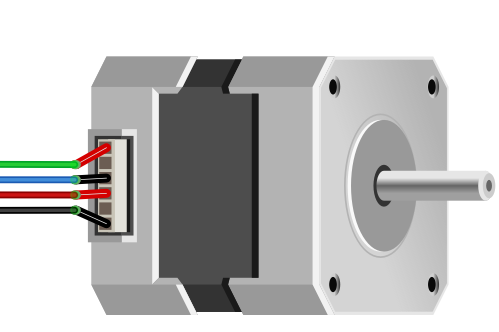
\includegraphics[width=0.8\linewidth, height=5cm]{Chapter_4/wires_jutting_out.png}
  \caption{Different coloured wires jutting out from a stepper motor}
  \label{fig:wires_out}
 \end{subfigure}

 \caption{Illustration representing the coils of a stepper motor and their equivalent coloured annotation}
 \label{fig:coil_representation}

\end{figure}

The exact terminology for the wires and their connection with the dedicated pins is better represented in table \ref{tab:mccons}. \par

Apart from the wire colour, the length of the wires from stepper motors is also to be taken into account while designing the project. It should be noted that the stepper motor responsible for the movement of the X-axis will be stationery itself. So the four leads/wires from it can be cut to length to just match or exceed its (the motor) distance from the CNC shield. This will ensure proper wire management and avoid inter looping and tangling between the wires in any circumstances. However, at the same time, it should be noted that the stepper motor responsible for the movement of the Y-axis will be mobile. So there is a high chance that they may get tangled amongst themselves and severe the connections between the motor and the CNC shield during actual operation. Therefore it is recommended that they are cut to a length equal to the maximum possible linear displacement of the tooltip in the Y-direction. If the shield is placed at half the maximum possible displacement in either of the axes then wires from both the stepper motors are supposed to be cut to a length just exceeding this value. However, in general, the wires associated with the stepper motor of the Y-axis are supposed to be tauter as well as more flexible as compared to the ones associated with the X-axis. \par

Also apart from the above conventions, thin wires are supposed to be always wrapped in insulating heat shrink material to avoid wear and tear from repeated use cycles. A representative illustration has been given below (although they have not been used as of now). \par

\begin{figure}[h]
 \centering
 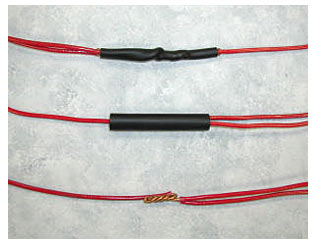
\includegraphics[scale = 0.7]{Chapter_4/heat_shrink.jpg}
 \caption{(From bottom to top) naked wire junction, heat shrink tubing placed on the junction and the shrunk tubing on application of heat}
 \label{fig:shrink}
\end{figure}

The stepper motor wires which are supported by loose jumper headers at the ends for interfacing purposes should preferably be soldered to the female headers on the CNC shield at the end once the entire design is finalised.

\subsubsection*{Wires related to power supply based connections}

\textit{This section is relevant because no customised universal PSU was designed for this project.}

The AC/DC adapter for the portable electric drill should be long if possible or should be used with an extension cord because the continuous operation of the drill requires that the wire is taut at all times yet it should not be too taut that a miniature movement shall severe the connection. At the same time, the adapter plug should be tight. \par

Similarly, single-stranded wires should suffice for the power connection of the CNC shield but should be properly insulated with heat shrink tubing after the pair of ends are screwed tightly into the input DC jack of the CNC shield. Even better, double-stranded wires could be used for this purpose eliminating the need for insulating tubing. \par

A USB Type-A to Type-B cable is required to interface an Arduino with a programming device. Both the ends should be equally tight which would prevent probable loss of connection during the phase of flashing a program onto the controller. This would handle both the power supply and programming requirements of the microcontroller development board. If the power supply is to be provided by means of the onboard DC jack then it should be ensured that the input side fits snugly into the jack.
